\documentclass[class=report,crop=false, 12pt]{standalone}
\usepackage[screen,nosolutions]{../scratch}

%\usepackage[print]{../scratch}
%\usepackage[screen]{../scratch}


\begin{document}


\titre[S]{Premiers pas}
%===============================

\insertvideo{onJG9sLbtNE}{Premiers pas -- Activité 1}

\insertvideo{4rdLxPcYMZ4}{Premiers pas -- Activité 2}

\insertvideo{jK29YG6WPgw}{Premiers pas -- Activité 3}

\bigskip
\bigskip


\begin{activite}

Commençons par déplacer le chat Scratch.

\begin{enumerate}
  \item
  \begin{itemize}
    \item Commence par déposer le bloc \og Quand le drapeau vert est cliqué \fg{} sur la partie droite.
    \item Puis colle juste au-dessous de ce bloc, le bloc \og Avancer de 10 \fg{}.
    \item Clique plusieurs fois sur le drapeau vert. 
  \end{itemize}

Scratch devrait avoir avancé !

\begin{center}
  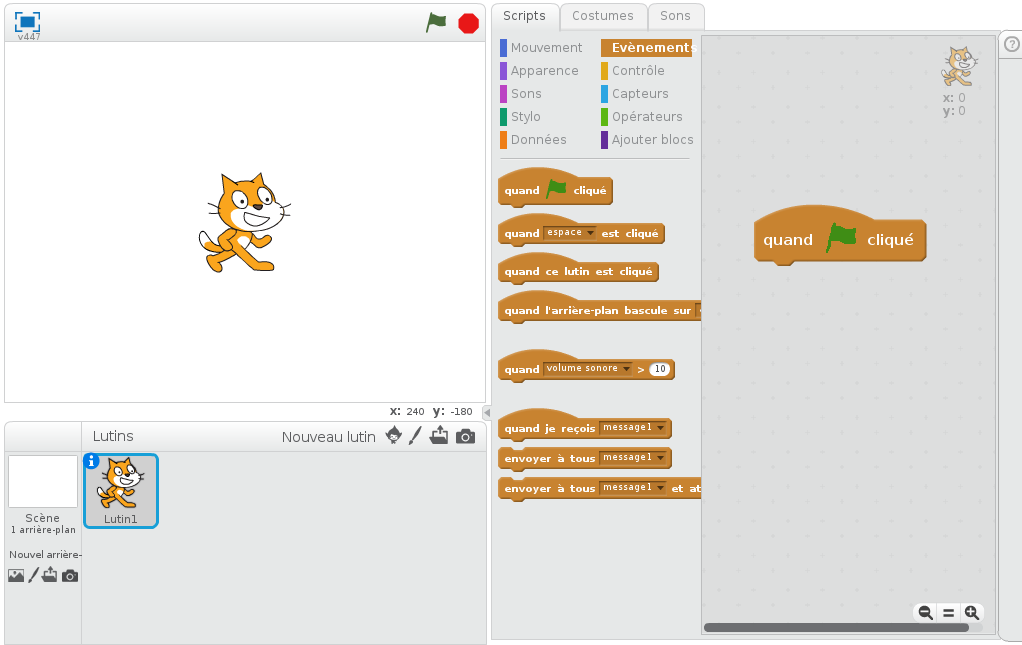
\includegraphics[scale=\scaleecran]{ecran-01-ex1a}

  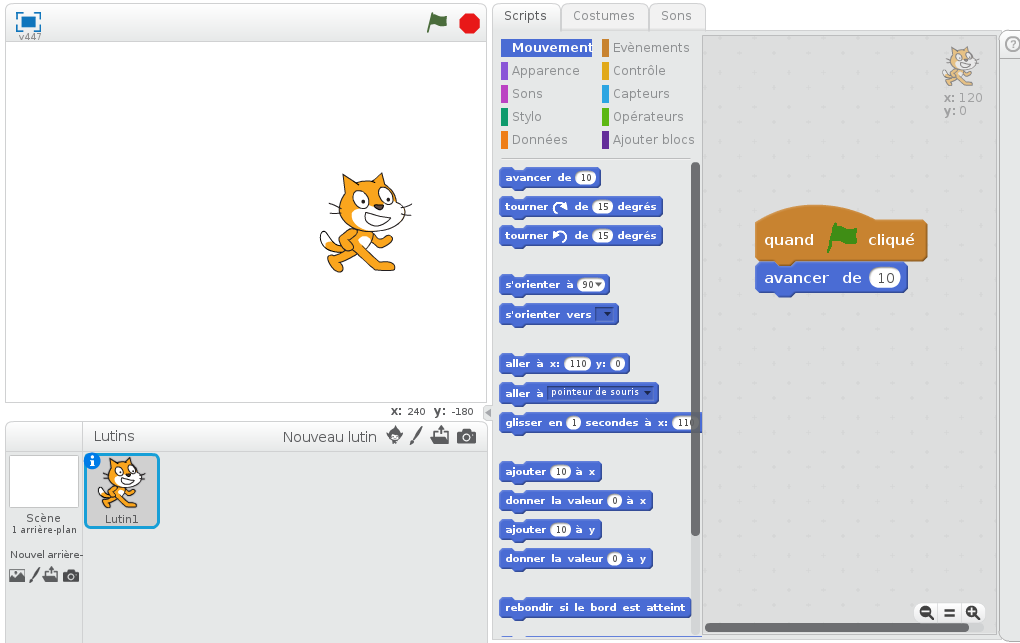
\includegraphics[scale=\scaleecran]{ecran-01-ex1b}
\end{center}  
  
  
Les deux blocs à positionner :
\begin{center}
  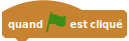
\includegraphics[scale=\scalebloc]{bloc-01-ex1a}
  \qquad\qquad
  
\includegraphics[scale=\scalebloc]{bloc-01-ex1b}
\end{center}    
  
  Il y a plusieurs problèmes : Scratch finit par être coincé à droite de l'écran, on aimerait qu'il revienne au départ, on aimerait aussi tracer son chemin.
  
  
  \item Pour que tout le monde démarre dans la même position à chaque fois que le drapeau vert est cliqué, commence toujours par les blocs suivants avant d'ajouter tes propres instructions :
  
  \begin{itemize}
    \item Quand le drapeau vert est cliqué
    \item Aller à $x = 0$, $y = 0$
    \item S'orienter à 90\textdegree\ (vers la droite)
    \item Effacer tout
    \item Stylo en position d'écriture
  \end{itemize}  
  
  Positionne ces blocs, puis fais avancer Scratch ! 
  
\begin{center}
  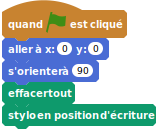
\includegraphics[scale=\scalebloc]{bloc-01-ex1c}
\end{center}   

  \item Voici ton premier programme :
  \begin{itemize}
    \item Fais avancer Scratch de 50 pas
    \item Fais une pause d'une seconde
    \item Fais encore avancer Scratch de 50 pas, puis une pause
    \item Fais avancer Scratch de 50 pas une dernière fois
  \end{itemize}
  
\myfigure{0.9}{
\tikzinput{ecran-01-ex1}
} 

\end{enumerate}
 
\end{activite}


\begin{activite}

Trace la figure suivante représentant la lettre \og G \fg{}.

\begin{center}
\begin{minipage}{0.3\textwidth}
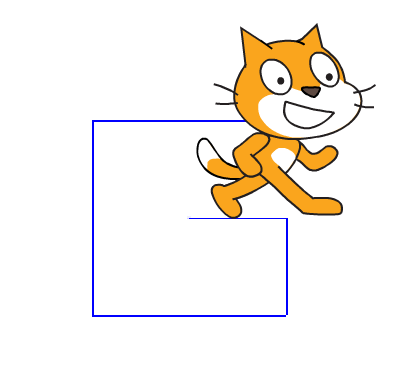
\includegraphics[width=\textwidth]{ecran-01-ex2}
\end{minipage}
\begin{minipage}{0.3\textwidth}
\myfigure{0.5}{
\tikzinput{ecran-01-ex2a}
} 
\end{minipage}
\begin{minipage}{0.3\textwidth}
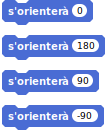
\includegraphics[scale=\scalebloc]{bloc-01-ex2}
\end{minipage}
\end{center}

Utilise seulement le bloc \og Avancer \fg{} et des blocs \og S'orienter à ... \fg{} pour te diriger vers le haut ($0$\textdegree), vers le bas ($180$\textdegree), vers la droite ($90$\textdegree) ou vers la gauche ($-90$\textdegree).

\bigskip

\textbf{Bonus.} 
Si tu es motivé, trace le symbole \og arobase \fg{}  \at :
\myfigure{1}{
\tikzinput{ecran-01-ex2b}
} 
 
\end{activite}


\begin{activite}

Trace la figure suivante réprésentant la lettre \og L \fg{}.

\begin{center}
\begin{minipage}{0.3\textwidth}
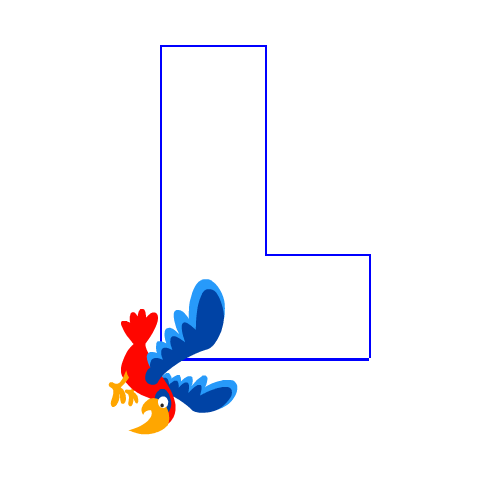
\includegraphics[width=\textwidth]{ecran-01-ex3}
\end{minipage}
\begin{minipage}{0.3\textwidth}
\myfigure{0.5}{
\tikzinput{ecran-01-ex3a}
} 
\end{minipage}
\begin{minipage}{0.3\textwidth}
  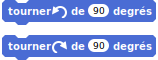
\includegraphics[scale=\scalebloc]{bloc-01-ex3}
\end{minipage}  
\end{center} 

Utilise seulement le bloc \og Avancer \fg{} et le bloc \og Tourner vers la droite de $90$\textdegree \fg{} pour tourner d'un quart de tour à droite, ou le bloc \og Tourner vers la gauche de $90$\textdegree \fg{} pour tourner d'un quart de tour à  gauche.

\bigskip

\textbf{Bonus 1.} Dans l'onglet \og Costumes \fg{}, choisis l'apparence que tu veux pour remplacer le chat.

\textbf{Bonus 2.} Si tu as le temps, trace le symbole d'un point d'interrogation.


\myfigure{1}{
\tikzinput{ecran-01-ex3b}
} 

\end{activite}


\ifx \displaysolutions \myzero
\else
\begin{code}
\onesolution{Premiers pas}{Activité 1}{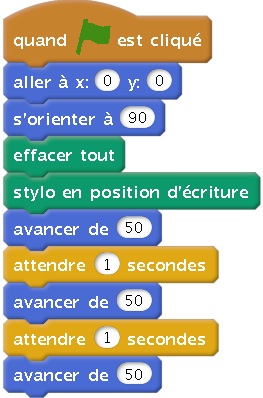
\includegraphics[scale=\scalesolution]{code-01-ex1}}
\onesolution{Premiers pas}{Activité 2}{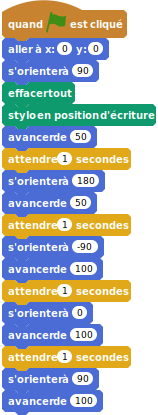
\includegraphics[scale=\scalesolution]{code-01-ex2}}
\onesolution{Premiers pas}{Activité 3}{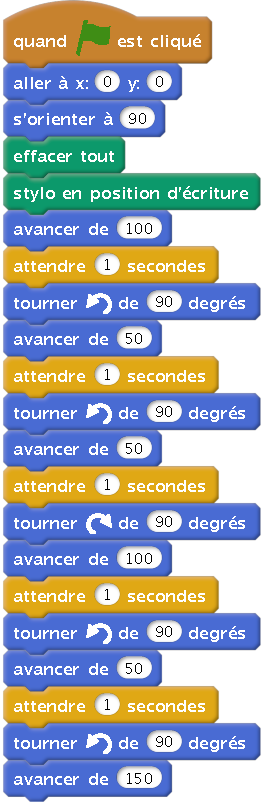
\includegraphics[scale=\scalesolution]{code-01-ex3}}
\end{code}
\fi



\end{document}


